%Kelompok5OS
%Dika Sukma Pradana
%Iqbal Hambali
%Evietania Sujadi
%Liyana Majdah Rahma


\section{VPython}
\subsection{Definisi}
		\begin{enumerate}
			\item VPython adalah bahasa pemrograman Python ditambah modul grafis 3D yang disebut Visual. VPython memungkinkan pengguna untuk membuat objek seperti bola dan kerucut dalam ruang 3D dan menampilkan objek-objek ini di windows. Ini membuatnya lebih mudah untuk membuat visualisasi sederhana, memungkinkan pemrogram untuk lebih fokus pada aspek komputasi dari program mereka. Kesederhanaan VPython telah menjadikannya alat untuk ilustrasi fisika sederhana, terutama dalam pengaturan pendidikan.
		\end{enumerate}
\subsection{Sejarah}
		\begin{enumerate}
			\item Pada tahun 1985, bahasa pemrograman cT diciptakan oleh para peneliti di Carnegie Mellon University. Kontributor untuk proyek ini termasuk David Andersen, Bruce Sherwood, Judith Sherwood, dan Kevin Whitley. Bahasa pemrograman cT sebagian besar dihasilkan dari TUTOR (1965) dan bahasa pemrograman MicroTutor (1977). Meskipun cT memiliki banyak aplikasi, penggunaan utamanya adalah grafik 2D untuk pengaturan ruang kelas. cT digunakan untuk banyak tujuan, tetapi ceruk utamanya adalah penciptaan program untuk pendidikan. Banyak program pendidikan pemenang penghargaan ditulis dalam cT (lihat VISQ), khususnya di bidang fisika. Pada tahun 1997, para siswa di Carnegie Mellon diajari cT dalam kursus pengantar fisika baru yang dibuat oleh Ruth Chabay dan Bruce Sherwood.
			\item Pada tahun 1985, bahasa pemrograman dibuat oleh para peneliti di Carnegie Mellon University. Kontributor untuk proyek ini termasuk David Andersen, Bruce Sherwood, Judith Sherwood, dan Kevin Whitley. Bahasa pemrograman cT sebagian besar dihasilkan dari TUTOR (1965) dan bahasa pemrograman MicroTutor (1977). Meskipun cT memiliki banyak aplikasi, penggunaannya adalah grafik 2D untuk konfigurasi ruang kelas. untuk banyak tujuan, tetapi ceruk mulia adalah penyediaan program untuk pendidikan. Banyak program pendidikan pemenang ditulis dalam cT (lihat VISQ), khususnya di bidang fisika. Pada tahun 1997, siswa di Carnegie Mellon mengajar cT dalam pengenalan fisika baru yang dibuat oleh Ruth Chabay dan Bruce Sherwood.
			\item 1997: Ketika di Carnegie Mellon, setelah menulis banyak buku tentang pengenalan dan magnet listrik, Ruth Chabay dan saya mengajarkan pengenalan "mekanika modern" untuk pertama kalinya, termasuk memiliki model komputasi siswa, menggunakan bahasa cT yang telah saya buat, sesuatu yang sedikit seperti Basic yang bagus, dengan built-in 2D graphics, tetapi berjalan dalam lingkungan windowing pada workstation Unix, Macintosh, dan Windows (general direction cT). c Berdasarkan TUTOR sistem pendidikan komputer berbasis PLATO (lihat halaman rumah untuk membahas sejarah sistem PLATO).
			\item 1998: Kami memiliki siswa yang luar biasa di kelas mekanik kami, David Scherer. Saat di sekolah menengah ia memimpin tim teman-temannya untuk membuat game 3D yang kemudian memenangkan hadiah nasional. Dia tertarik bahwa cT telah memungkinkan siswa untuk menulis model komputasi yang bekerja di semua platform, tetapi dia melihat pendekatan yang lebih kuat yang akan mendukung 3D.
			\item 2000: Kami meninggalkan cT, dan pada musim semi Scherer menciptakan VPython, dengan Ruth dan saya sangat terlibat dalam desain dan pengujian. Banyak programmer yang kuat tidak tertarik atau sabar terhadap programmer pemula, tetapi Scherer melihatnya sebagai tantangan yang menarik bagaimana membuat animasi 3D terprogram dapat diakses oleh pemula. Jawabannya adalah membuat animasi 3D navigasi real-time sebagai efek samping dari perhitungan, mengangkat tugas besar dari pundak pemula. Tentu saja ini juga merupakan manfaat besar bagi para programmer yang canggih juga. Versi asli VPython sekarang disebut "Klasik" VPython. Ini membutuhkan menginstal Python, "visual" modul, dan editor program yang ditingkatkan berdasarkan editor IDLE yang datang dengan Python. Pada musim gugur tahun 2000 kami mulai memiliki siswa menggunakan VPython untuk melakukan pemodelan komputasi dalam kursus kami.
			\item 2002-2006: Jonathan Brandmeyer, seorang mahasiswa teknik di NCSU, memberikan kontribusi besar kepada VPython 3. Dia memperkenalkan penggunaan pustaka C ++ Boost untuk merekatkan inti VPython, diimplementasikan dalam kode C ++ berulir, ke komponen yang ditulis dengan Python, dan membuat installer yang dapat dikonfigurasi secara otomatis untuk Linux. Dalam 16 tahun sejarah VPython hanya tiga orang yang memberikan kontribusi besar pada kode C ++ kompleks, Scherer, Brandmeyer, dan saya.
		\end{enumerate}
\subsection{Kegunaan Vpython}
		\begin{enumerate}
			\item VPhython adalah alat render sederhana untuk objek 3D dan grafik. Penggunaan utamanya dalam pendidikan, tetapi juga digunakan dalam pengaturan komersial atau penelitian. VPython pertama kali digunakan dalam mata kuliah pengantar fisika di Carnegie Mellon dan kemudian menyebar ke universitas lain dan akhirnya sekolah menengah atas, terutama yang berhubungan dengan Materi & Kurikulum Interaksi.
			\item Perkembangan terkait karena David Scherer dan Bruce Sherwood adalah GlowScript, yang memungkinkan untuk menulis dan menjalankan program VPython di browser, termasuk di perangkat seluler, berkat kompilasi RapydScript Python-ke-JavaScript, yang dibuat oleh Alexander Tsepkov. Program dapat ditulis, dijalankan, dan disimpan di glowscript.org, dan kode dikompilasi-ke-JavaScript dapat diekspor dan disematkan di halaman web seseorang. John Coady telah membuat versi ivisual untuk digunakan dalam IPython, sekarang lingkungan Jupyter, menggunakan pustaka grafis GlowScript WebGL untuk merender output 3D dalam notebook IPython / Jupyter. Rhett Allain di blog Wired-nya menunjukkan contoh penggunaan Trinket untuk menyematkan kode sumber VPython yang dapat diedit dan eksekusi 3D di halaman webnya sendiri.
		\end{enumerate}
\subsection{Kelebihan VPython}
		\begin{enumerate}
			\item Tidak ada langkah kompilasi dan tautan (tautan) sehingga perubahan kecepatan dalam sistem yang dibuat ditambah aplikasi.
			\item Tidak ada deklarasi tipe data yang rumit sehingga program menjadi lebih sederhana, lebih pendek, dan lebih fleksibel.
			\item Manajemen memori otomatis adalah kumpulan sampah memori sehingga dapat menghindari enkripsi kode.
			\item Jenis data dan tingkat operasi yang tinggi adalah kecepatan dari sistem yang dibuat menggunakan jenis objek yang ada.
		\end{enumerate}
\subsection{Kekurangan VPython}
		\begin {enumerate}
			\item Beberapa tugas berada di luar jangkauan python, seperti bahasa pemrograman dinamis lainnya, python tidak secepat atau seefisien statis, tidak seperti bahasa pemrograman kompilasi bahasa C yang serupa.
			\item Karena python adalah seorang interpreter, python bukanlah alat terbaik untuk memperkenalkan komponen kinerja yang penting.
			\item Python tidak dapat digunakan sebagai dasar untuk mengimplementasikan bahasa pemrograman untuk beberapa komponen, tetapi berfungsi dengan baik ketika bagian depan skrip mencarinya.
			\item Python memberikan efisiensi dan fleksibilitas dari tradeoff dengan tidak memberikannya secara luas. Python mempersiapkan bahasa pemrograman optimasi untuk kegunaan, bersama dengan alat yang diperlukan untuk mengintegrasikannya dengan bahasa pemrograman lainnya.
		\end{enumerate}
\subsection{Variabel dan Tipe Data Pada vpython}	
		\begin{enumerate}
			\item Variabel adalah memori yang dicadangkan untuk menyimpan nilai-nilai. Artinya dengan variabel, kita dapat menyimpan nilai dalam program yang nantinya akan kita tampilkan. Namun variabel hanya bersifat sementara. Yaitu hanya menyimpan ketika program dijalankan. Jika sudah ditutup, maka nilai didalam variabel tersebut akan terhapus otomatis.
			\item Jenis Variabel Pada Python tidak serumit bahasa pemrograman lain. Karena pada bahasa pemrograman python, jenis variabel tidak ditentukan dengan tipe data yang ada. variabel pada python hanya kita buat dengan tulisan sesuai dengan selera kita. Jadi tidak perlu memusingkan diri dengan masalah variabel.
			\item Tipe Data adalah jenis nilai yang dapat ditampung variabel, dan memiliki jenis-jenis tertentu. Artinya tipe data merupakan tipe / jenis dari suatu value, yang nantinya akan disimpan ke dalam variabel.Dari pengertian ini, kita bisa mengetahui bahwa variabel dan tipe data adalah hal yang bersangkutan. Untuk bahasa pemrograman lain memang benar. Tapi untuk python itu tidak sepenuhnya benar.  
			\item Tipe Data di Python memiliki berbagai jenis. Antara lain huruf, karakter, angka, boolean dan list (kelompok). tipe data tersebut nantinya disimpan ke dalam variabel di program python sesuai dengan jenisnya. 
		\end{enumerate}
		\begin{verbatim}
			from visual import * #import the visual module

			rod = cylinder(pos=(0,2,1), axis=(5,0,0), radius=1)
		\end{verbatim}
		\begin{figure}[ht]
					\centerline{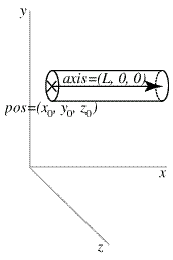
\includegraphics[width=1\textwidth]{figures/OSS.jpg}}
				\caption{Coding}
			\label{Vphython}
		\end{figure}
	Gambar \ref{Vphython} Gambar.
		\begin{verbatim}
			from visual.graph import * # import graphing features
			from numpy import arange, cos, exp

			funct1 = gcurve(color=color.cyan) # a connected curve object

			for x in arange(0., 8.1, 0.1): # x goes from 0 to 8
			funct1.plot(pos=(x,5.*cos(2.*x)*exp(-0.2*x))) # plot
		\end{verbatim}
		
\cite{scherer2000vpython}
\cite{sherwood2011vpython}
\cite{roberts2004teaching}
\cite{marciuc2016using}

\subsection { Percabangan bahasa pemrograman di python}
		 
		 \begin {enumerate}
			\item Percabangan di Python terdapat 4 macam.. Yang mana percabangan tersebut digunakan pada bahasa pemrograman python. Berikut ini merupakan macam-macam percabangan pada bahasa pemrograman python :
			\item IF Statement
			\item IF - ELSE Statement
			\item IF - ELIF - ELSE Statement
			\item IF Bersarang(Nested IF)
			\end {enumerate}
			
			\begin {enumerate}
			\item Berikut ini merupakan penjelasannya dari macam-macam percabangan pada bahasa pemrograman python.
			\item IF Statement Fungsi IF pada python adalah untuk memberikan kondisi tertentu pada program supaya program bisa berjalan sesuai dengan kondisi tersebut. Fungsi yang dipakai adalah IF(jika). Dengan fungsi tersebut, kita dapat lebih leluasa dalam pemrograman python.
			\item IF - ELSE Statement Fungsi IF - ELSE pada python adalah untuk memberikan 2 kondisi yang mana kedua kondisi tersebut bersifat terbalik. artinya apabila kondisi pertama tidak memenuhi, maka akan muncul kondisi kedua(ELSE) secara otomatis.
			\item IF - ELIF - ELSE Statement Jika sebelumnya hanya memiliki satu kondisi, disini ada tambahan Elif pada python. ELIF adalah perintah pada program python untuk menammbah kondisi. Dalam hal ini, kondisi pada ELIF bisa digunakan berkali - kali.
			\item IF Bersarang(Nested IF) IF Bersarang merupakan kondisi yang didalamnya terdapat kondisi lagi. Misalkan keputusan kita setelah SMA, ada dua pilihan. Yaitu Kuliah atau Kerja. Jika kita memilih kuliah, ada pilihan lagi didalamnya, yaitu daftar di kampus mana. dan seterusnya. Hal tersebut bisa kita bahasakan denga IF dalam IF.
\end {enumerate}
